Vi valgte derfor i starten af sprint 2 at dele den op. Derudover delte vi ogs� andre store userstories op...

Vi lavede en ny burndown som viste mandetimer per mandedage. \\
Vi splittede vores userstories og produktbacklog bedre op, samt lavede nye estimater i b�de storypoint og mandetimer p� hver enkelt userstory. Derudover satte vi ogs� tidsestimater p� vores tasks for bedre at v�re i stand til at afslutte tasks og at kunne tegne vores burndown ned. \\
Sprintet kom i h�j grad til at handle om userstories for at lave database samt kobling af database og foodmap.

\subsection*{Velocity}

\subsection*{Planl�gning}

\subsection*{Xp og scrum praktikker}

\subsection{Produkt review}

\subsubsection*{Konklusion af review}

\subsection*{Retrospektive}

\subsubsection*{Ting der gik godt}

\subsubsection*{Mindre godt}

\subsubsection*{Hvad �ndrer vi til n�ste sprint}

\subsection*{Product backlog}
Backlog lavet den 9.12.2013 i starten af sprint 2. \\
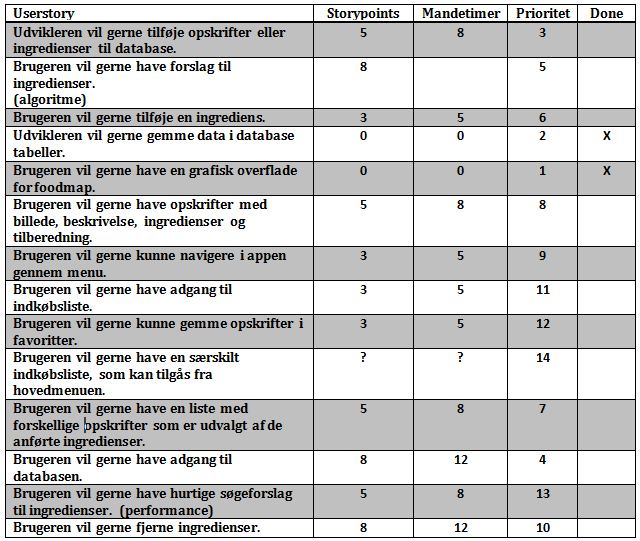
\includegraphics[scale=0.60]{includes/billeder/productbacklog_sprint2.png}